\scanpage{62}
\margin{\unsure{l'image de $q$ est inversible}}
\diagram{\begin{tikzcd}[ampersand replacement=\&]
\widehat A_p\arrow[r,"q\widehat A_p"] \& A_{[p,q]}\\
A\arrow[u]\arrow[r] \& \widehat A_q\arrow[u,"\text{hom local}"']
\end{tikzcd}}
\[\unsure{\mathrm{comm}}\]
\diagram{\begin{tikzcd}[ampersand replacement=\&,column sep=small]
\& A_{[p,q,\unsure{r|v}]}\&\\
A_{[p,q]}\arrow[ur]\&\& A_{[q,r]}\arrow[ul]\\
A_{[p]}\arrow[u]\& A_{[q]}\arrow[ul]\arrow[ur]\& A_{[r]}\arrow[u]\\
\& A_p\arrow[ul]\arrow[u]\arrow[ur,"\text{\unsure{complété par $r$}}"']\&
\end{tikzcd}}
\figure{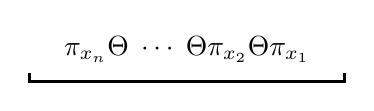
\begin{tikzpicture}
\node at (2,0.4) {$\pi_{x_n}\Theta\;\cdots\;\Theta\pi_{x_2}\Theta\pi_{x_1}$};
\draw[line width=1.3pt] (0,0.1)--(0,0)--(4,0)--(4,0.1);
\end{tikzpicture}}
\[p\supset q\supset r\]
\diagram{\begin{tikzcd}[ampersand replacement=\&]
A_{[p,q]}\\
A_q\arrow[u,"\text{local plat dim relative 0}"]
\end{tikzcd}}
\[ A_q/qA_q \]
\margin{\unsure{il y a donc un corps} \unsure{non commutatif} de dim 1, savoir $A/q$, \unsure{dont on prend le complété} \unsure{-----}}
\[p\supset q\supset r\]
\figure{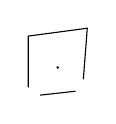
\begin{tikzpicture}[scale=.5]
\draw (0,0)--(0,1.3)--(1.5,1.5)--(1.4,.2);\draw (.3,-.2)--(1.2,-.1);\fill (.75,.5) circle (.035);
\end{tikzpicture}}
\diagram{\begin{tikzcd}[ampersand replacement=\&]
\widehat A_p\\ A_p\arrow[u]
\end{tikzcd}}
\[
A_{[p,q]}\otimes_{A_q} A_{\deleted{\unsure{p}}r}/r^n A_r
\]
\[
\underbrace{A_{[p,q]}/r^n A_{[p,q]}}_{\text{dim 1}}\otimes A_r\deleted{\unsure{A_q}}
\]
\unsure{complété de}
\[A/\]
\diagram{\begin{tikzcd}[ampersand replacement=\&,column sep=small]
A_{[p_1,\ldots,p_{n-1}]}\arrow[rr,"\deleted{\unsure{R}}"]\&\& A_{[p_1,\ldots;p_n]}\\
\&\deleted{A_{[p_1}}\arrow[ur]\&\\
\&\widehat A_{p_1}\arrow[uur]\arrow[r,dash]\&\widehat A_{p_i}\arrow[uul]\arrow[r,dash]\&\widehat A_{p_n}\arrow[uul]
\end{tikzcd}}
\[A_{[p_1,\ldots,}\]
\figure{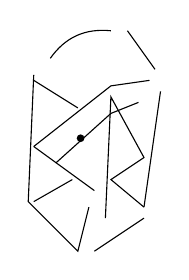
\begin{tikzpicture}[scale=.7]
\draw (0,2.8)--(-.1,.5)--(.8,-.4)--(1,.4);
\draw (.3,3.1) to[bend left] (1.4,3.6);\draw (1.7,3.6)--(2.2,2.9);
\draw (2.3,2.5)--(2,.4);\draw (1.1,-.4)--(2,.2);
\draw (0,2.7)--(.8,2.2);\draw (0,1.5)--(1.1,.7);\draw (0,.5)--(.7,.9);
\draw (0,1.5)--(1.4,2.6)--(2.1,2.7);\draw (.4,1.2)--(1.4,2.1)--(1.9,2.3);
\draw (1.3,.2)--(1.4,2.4)--(2,1.3)--(1.4,.9)--(2,.4);
\fill (.85,1.65) circle (.07);
\end{tikzpicture}}
\diagram{\begin{tikzcd}[ampersand replacement=\&]
\&\unsure{\mathcal C|C}\arrow[d]\&\\
{}\&\unsure{\text{Ch. Sat}|\text{An. Sat}}\arrow[l,dash dot,bend left=20]\&
\end{tikzcd}}
\figure{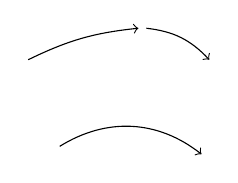
\begin{tikzpicture}
\draw[->] (0,1.2) to[bend left=10] (1.4,1.6);\draw[->] (1.5,1.6) to[bend left=20] (2.3,1.2);
\draw[->] (.4,.1) to[bend left=35] (2.2,0);
\end{tikzpicture}}
\diagram{\begin{tikzcd}[ampersand replacement=\&]
x_0\arrow[r,"\text{chaine saturée}"']\&x_n
\end{tikzcd}}
% archive sheet number: 61
